\section{Results}
\begin{frame}[fragile]{Results} 
\begin{center}
 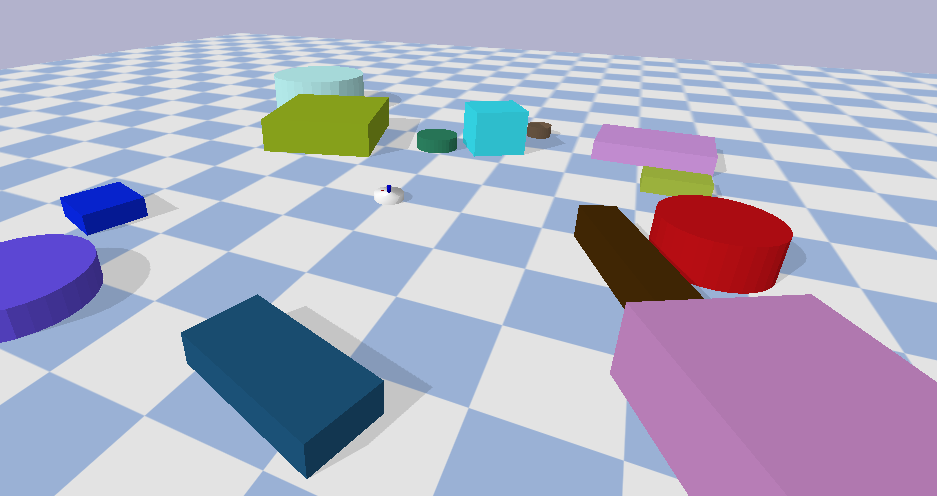
\includegraphics[width=0.8\textwidth]{figures/results/random1}
\end{center}
\end{frame}

\begin{frame}[fragile]{Results} 
\begin{center}
 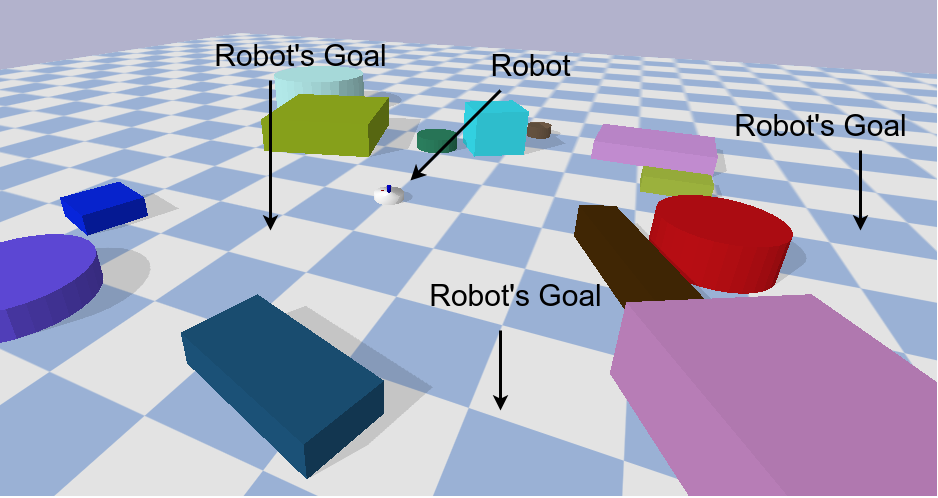
\includegraphics[width=0.8\textwidth]{figures/results/random1_with_target}
\end{center}
\end{frame}

\begin{frame}[fragile]{Results} 
\begin{figure}
  \centering
  \subfloat{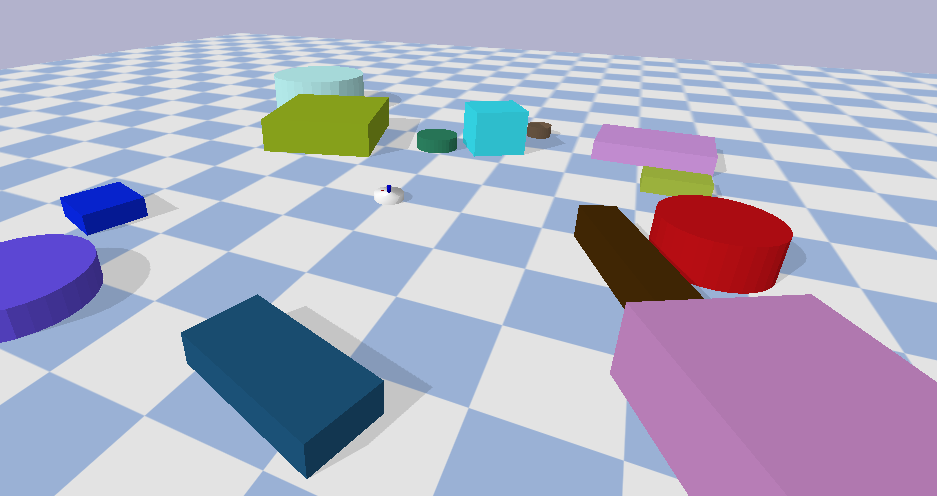
\includegraphics[width=0.48\textwidth]{figures/results/random1}}\quad
  \subfloat{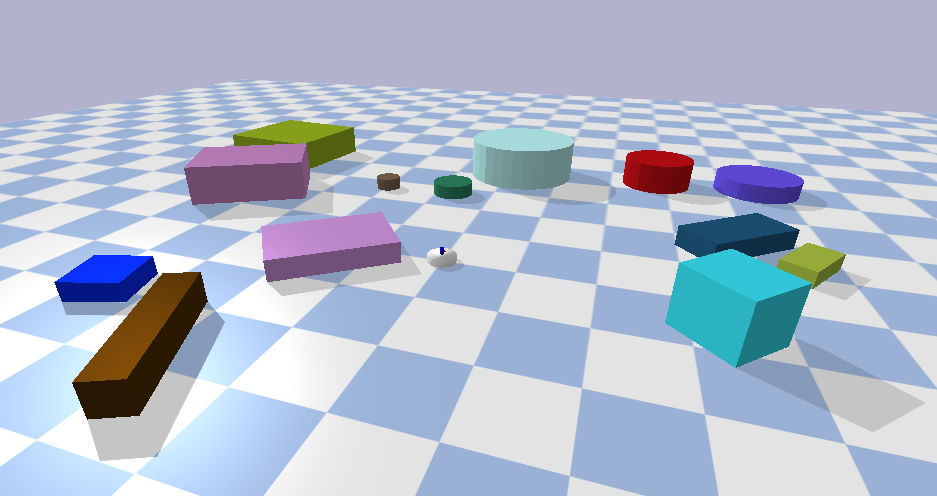
\includegraphics[width=0.48\textwidth]{figures/results/random2}}
\end{figure}
\end{frame}

\begin{frame}[fragile]{Results} 
\begin{figure}
  \centering
  \subfloat{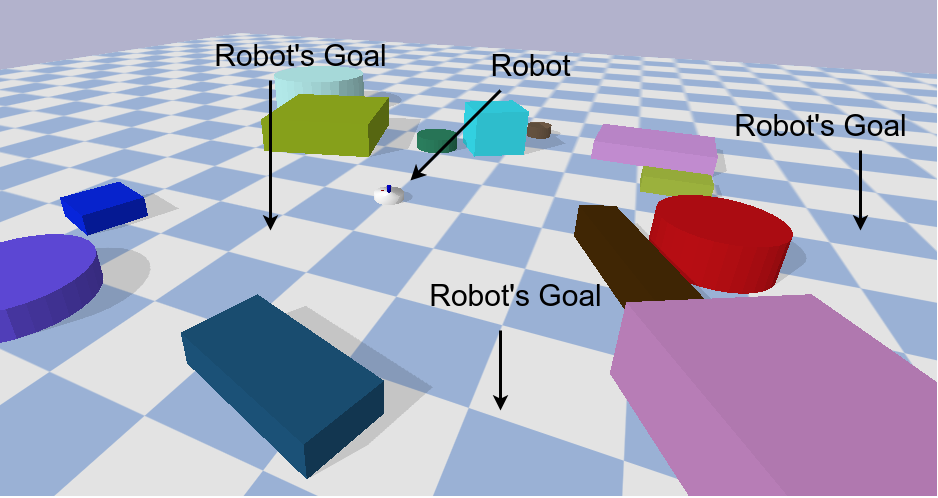
\includegraphics[width=0.48\textwidth]{figures/results/random1_with_target}}\quad
  \subfloat{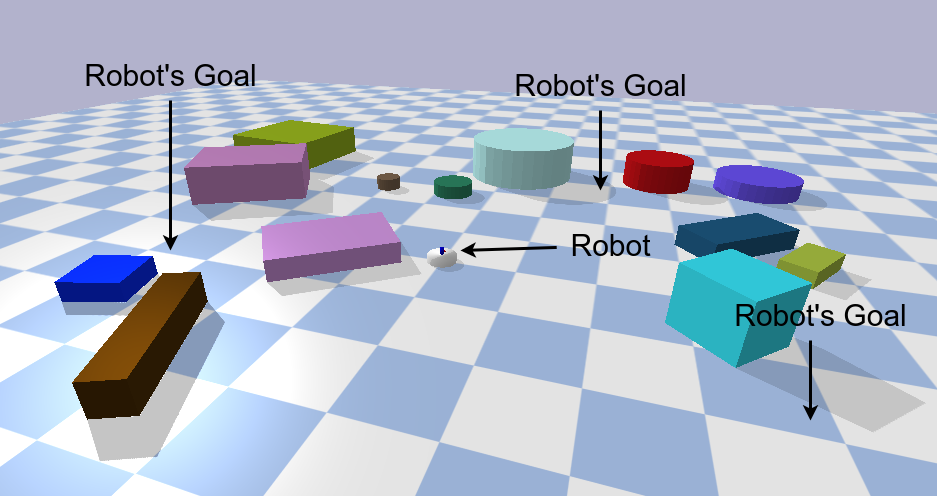
\includegraphics[width=0.48\textwidth]{figures/results/random2_with_target}}
\end{figure}
\end{frame}

% \begin{frame}[fragile]{Results} 
%   \begin{center}
%     \movie[width=0.8\textwidth, height=0.41\textwidth, autostart, poster]{}{figures/results/confetti.mp4}
%   \end{center}
% \end{frame}

\begin{frame}[fragile]{Results} 
\begin{table}[H]
    \centering
    \begin{tabular}%
    {l | p{0.3cm} p{0.3cm} p{0.3cm} p{0.3cm} p{0.3cm} p{0.3cm} p{0.3cm} p{0.3cm}p{0.3cm} p{0.3cm}}
  Run &  &   &  &  & Task &  &  &  &  & \\ \hline
  $\mathit{run}_1$ & 1 & 1  & 1 & 1 & 1 & 1 & 1 & 1 & 1 & 1\\
  $\mathit{run}_2$ & 1 & 1  & 1 & 1 & 1 & 1 & 1 & 1 & 1 & 1\\
  \quad\vdots &\vdots & \vdots  & \vdots & \vdots & \vdots & \vdots & \vdots & \vdots & \vdots & \vdots\\
  $\mathit{run}_{10}$ & 1 & 1  & 1 & 1 & 1 & 1 & 1 & 1 & 1 & 1\\\hline
    Tasks in experience & 0 & 1 & 2 & 3 &4 & 5 &6 & 7& 8  &9\\ 
    \end{tabular}
\end{table}


\end{frame}

\begin{frame}[fragile]{Results} 
\begin{table}[H]
    \centering
    \begin{tabular}%
    {l | p{0.3cm} p{0.3cm} p{0.3cm} p{0.3cm} p{0.3cm} p{0.3cm} p{0.3cm} p{0.3cm}p{0.3cm} p{0.3cm}}
    Task & 10 & 10  & 10 & 10 & 10 & 10 & 10 & 10 & 10 & 10\\
    Tasks in experience & 0 & 1 & 2 & 3 &4 & 5 &6 & 7& 8  &9\\ 
    \end{tabular}
\end{table}

\[\textrm{number of subtasks} = 10 * 10 * 3 = 300\]
\end{frame}


\begin{frame}[fragile]{Results} 
\begin{center}
  \hbox{\hspace{-0.7cm} 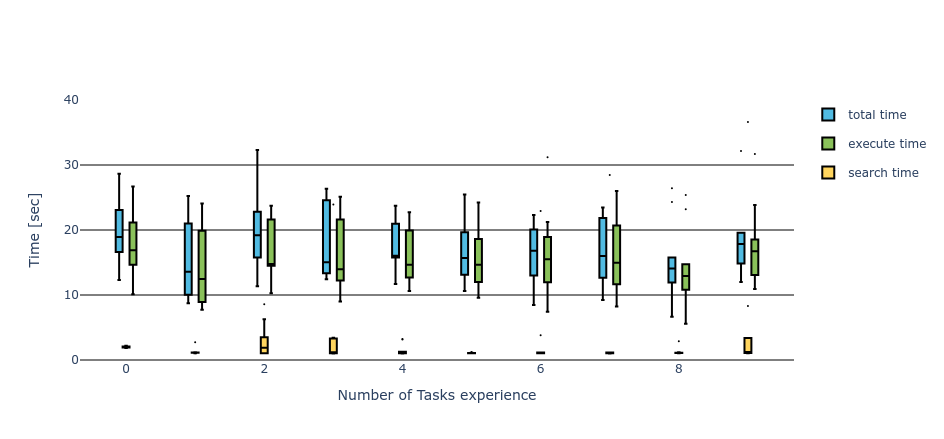
\includegraphics[width=1.05\textwidth]{figures/results/random_drive_time_k-graph} }
\end{center}
\end{frame}

\begin{frame}[fragile]{Results} 
\begin{center}
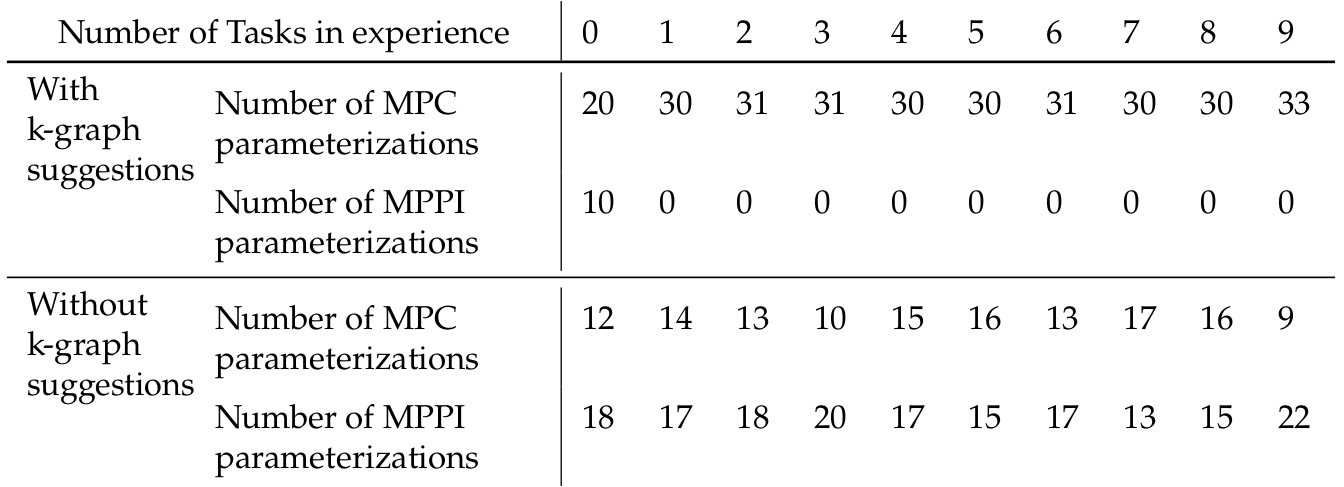
\includegraphics[width=1.0\textwidth]{figures/results/random_drive_para}
\end{center}
\end{frame}

\begin{frame}[fragile]{Results} 
\begin{center}
  \hbox{\hspace{-0.7cm} 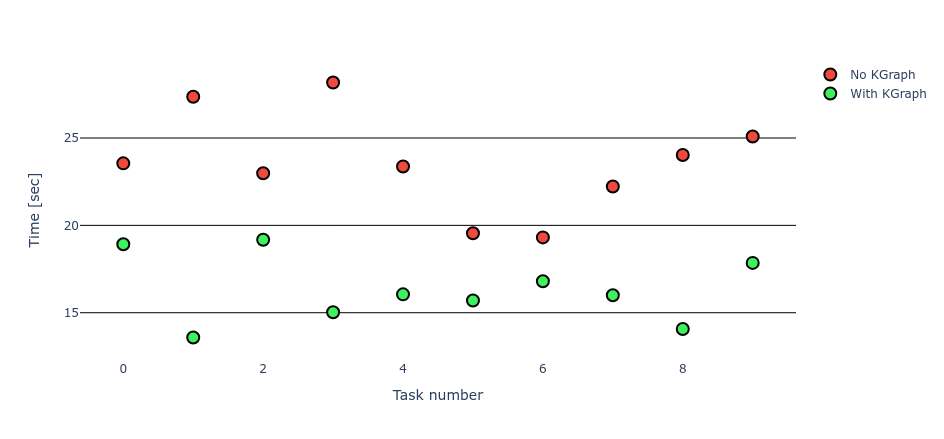
\includegraphics[width=1.05\textwidth]{figures/results/random_drive_time_vs}}
\end{center}
\end{frame}

\begin{frame}[fragile]{Results} 
\begin{center}
   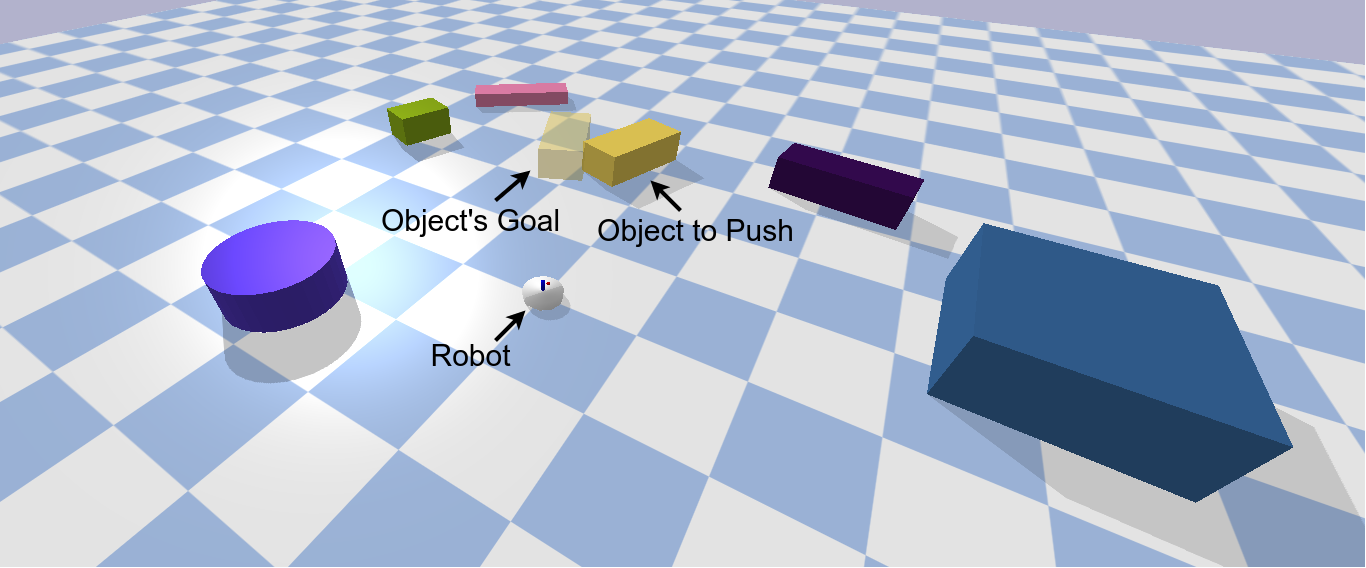
\includegraphics[width=1.0\textwidth]{figures/results/random_1.drawio}
\end{center}
\end{frame}


\begin{frame}[fragile]{Results} 
\begin{center}
  \hbox{\hspace{-0.7cm} 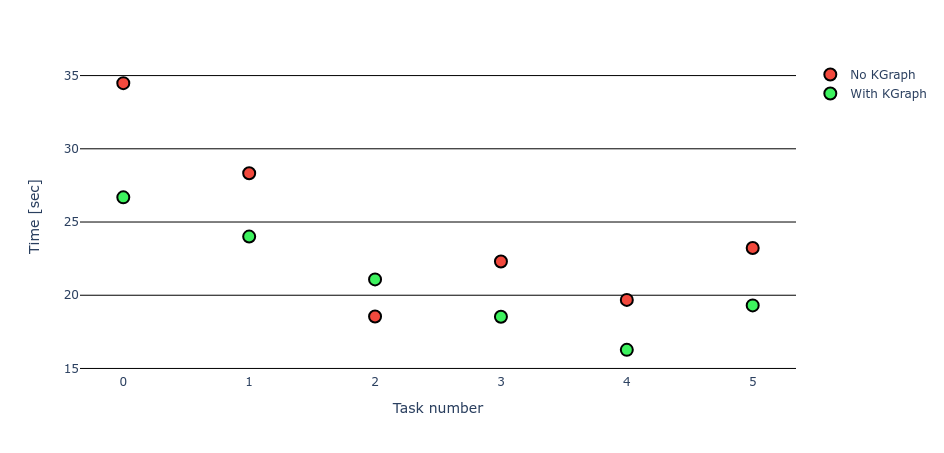
\includegraphics[width=1.1\textwidth]{figures/results/random_push_time_vs}}
\end{center}
\end{frame}


% \begin{frame}[fragile]{Results} 
  % \todo{success factor targets the prediction error, not really that otehr thingy}
% \end{frame}

\begin{frame}[fragile]{Results} 
\begin{center}
  \hbox{\hspace{-0.05\textwidth} 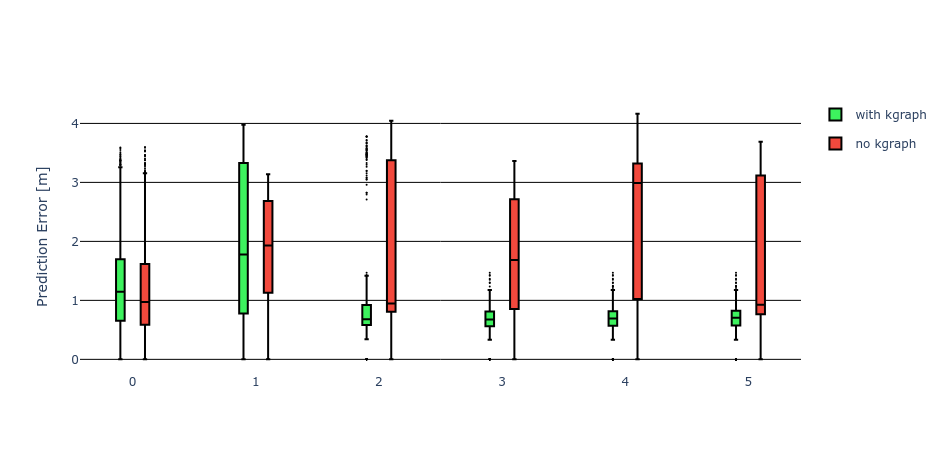
\includegraphics[width=1.1\textwidth]{figures/results/random_push_pe_vs}}
\end{center}
\end{frame}


\begin{frame}[fragile]{Results} 
\begin{center}
 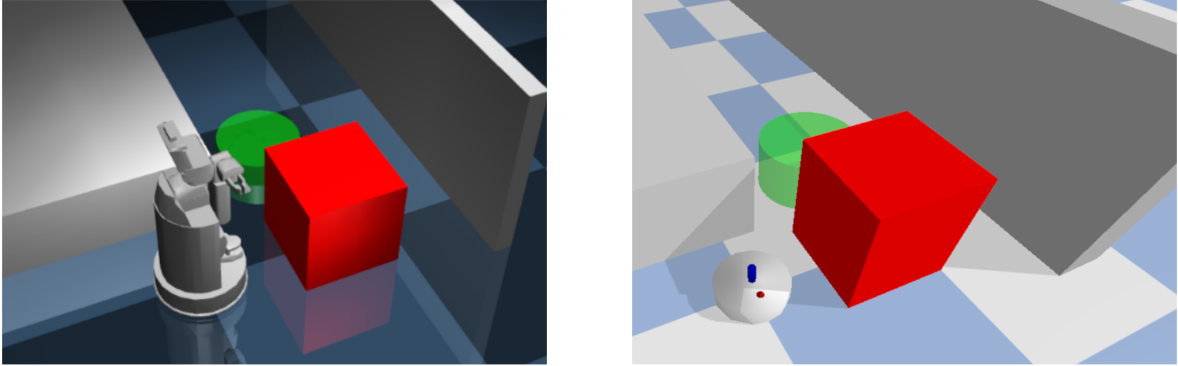
\includegraphics[width=1.0\textwidth]{figures/results/compare_sota}
\end{center}
\end{frame}


\begin{frame}[fragile]{Results} 
\begin{center}
 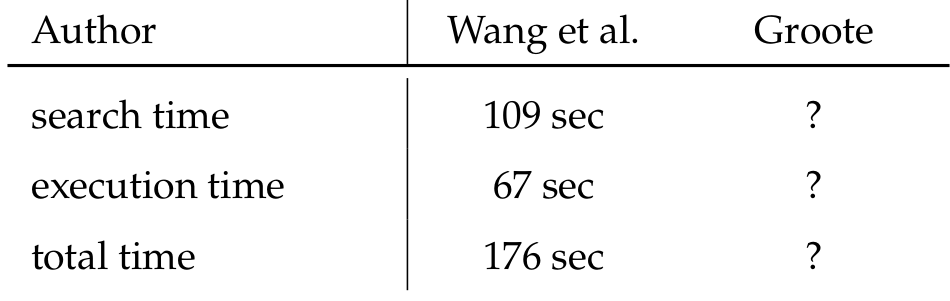
\includegraphics[width=0.7\textwidth]{figures/results/wang_groote_1}
\end{center}
\end{frame}

\begin{frame}[fragile]{Results} 
\begin{center}
 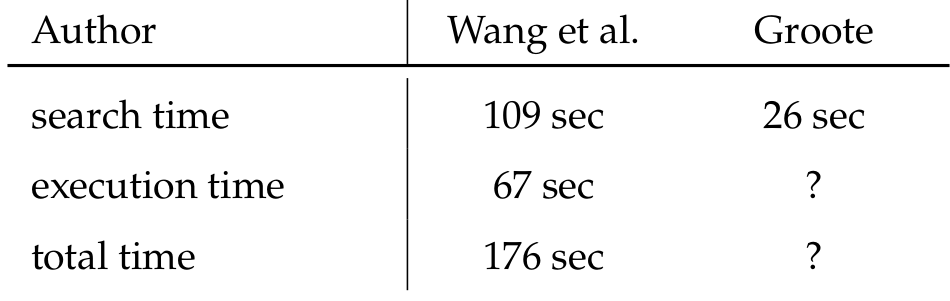
\includegraphics[width=0.7\textwidth]{figures/results/wang_groote_2}
\end{center}
\end{frame}
\begin{frame}[fragile]{Results} 
\begin{center}
 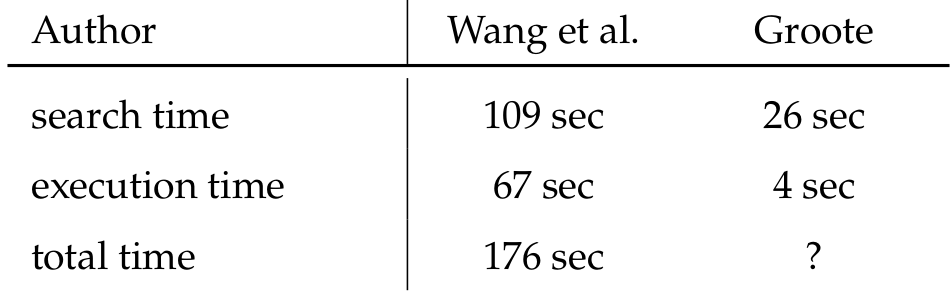
\includegraphics[width=0.7\textwidth]{figures/results/wang_groote_3}
\end{center}
\end{frame}
\begin{frame}[fragile]{Results} 
\begin{center}
 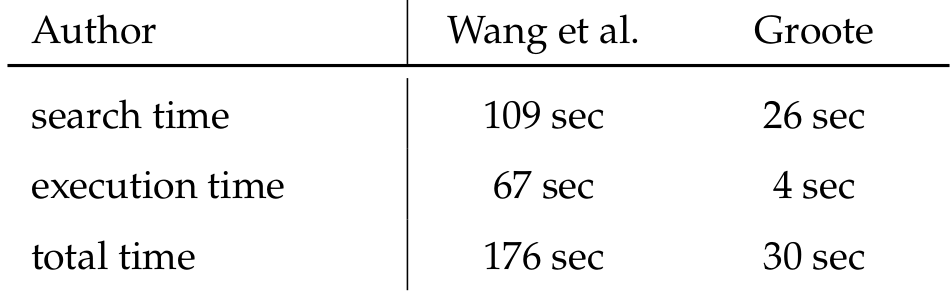
\includegraphics[width=0.7\textwidth]{figures/results/wang_groote_4}
\end{center}
\end{frame}





